% Overview: 4 storage modes — table taxonomy
\documentclass[tikz,border=4mm]{standalone}
\usepackage[T1]{fontenc}
\usepackage{lmodern}
% Shared TikZ styles for Flexograph table-layout diagrams.
% Include with % Shared TikZ styles for Flexograph table-layout diagrams.
% Include with % Shared TikZ styles for Flexograph table-layout diagrams.
% Include with \input{schema_styles} in each standalone figure.

\usetikzlibrary{shapes.multipart, arrows.meta, positioning, fit, calc, backgrounds}

% ── Colour palette ──────────────────────────────────────────────────
\definecolor{tblheader}{HTML}{2C3E50}   % dark blue-grey header bar
\definecolor{tblbody}{HTML}{ECF0F1}     % light grey table body
\definecolor{sentbg}{HTML}{D5DBDB}      % sentinel row shading
\definecolor{cgTemporal}{HTML}{AED6F1}  % column group: temporal
\definecolor{cgName}{HTML}{A9DFBF}      % column group: name
\definecolor{cgContact}{HTML}{F9E79F}   % column group: contact
\definecolor{cgLocation}{HTML}{F5CBA7}  % column group: location
\definecolor{cgContent}{HTML}{D2B4DE}   % column group: content
\definecolor{structClr}{HTML}{85929E}   % structural table border
\definecolor{propClr}{HTML}{2980B9}     % property table border
\definecolor{secClr}{HTML}{27AE60}      % secondary table border
\definecolor{arrowClr}{HTML}{7F8C8D}    % relationship arrows

% ── Node styles ─────────────────────────────────────────────────────
\tikzset{
  % Table header bar
  tblhdr/.style={
    rectangle, draw=tblheader, fill=tblheader,
    text=white, font=\sffamily\bfseries\footnotesize,
    minimum width=#1, minimum height=5mm, inner sep=2pt,
    align=center,
  },
  tblhdr/.default=38mm,
  % Table body (single cell / row)
  tblcell/.style={
    rectangle, draw=tblheader!40, fill=tblbody,
    font=\sffamily\scriptsize, minimum width=#1,
    minimum height=4.5mm, inner sep=2pt, align=center,
  },
  tblcell/.default=38mm,
  % Sentinel-row variant
  sentcell/.style={
    tblcell=#1, fill=sentbg,
  },
  sentcell/.default=38mm,
  % Column-group cell (coloured)
  cgcell/.style 2 args={
    tblcell=#1, fill=#2,
  },
  % Key column (narrower, left-aligned)
  keycell/.style={
    tblcell=#1, font=\sffamily\scriptsize\itshape,
  },
  keycell/.default=18mm,
  % Format annotation
  fmtlabel/.style={
    font=\sffamily\tiny\color{tblheader!70}, anchor=north west,
  },
  % Dashed grouping box
  groupbox/.style={
    rectangle, rounded corners=2pt, draw=#1, densely dashed,
    line width=0.6pt, inner sep=3pt,
  },
  groupbox/.default=structClr,
  % Relationship arrow
  relarrow/.style={
    -{Stealth[length=2.5mm]}, arrowClr, line width=0.5pt,
  },
  % Label for relationship
  rellabel/.style={
    font=\sffamily\tiny\color{arrowClr}, midway, fill=white, inner sep=1pt,
  },
}
 in each standalone figure.

\usetikzlibrary{shapes.multipart, arrows.meta, positioning, fit, calc, backgrounds}

% ── Colour palette ──────────────────────────────────────────────────
\definecolor{tblheader}{HTML}{2C3E50}   % dark blue-grey header bar
\definecolor{tblbody}{HTML}{ECF0F1}     % light grey table body
\definecolor{sentbg}{HTML}{D5DBDB}      % sentinel row shading
\definecolor{cgTemporal}{HTML}{AED6F1}  % column group: temporal
\definecolor{cgName}{HTML}{A9DFBF}      % column group: name
\definecolor{cgContact}{HTML}{F9E79F}   % column group: contact
\definecolor{cgLocation}{HTML}{F5CBA7}  % column group: location
\definecolor{cgContent}{HTML}{D2B4DE}   % column group: content
\definecolor{structClr}{HTML}{85929E}   % structural table border
\definecolor{propClr}{HTML}{2980B9}     % property table border
\definecolor{secClr}{HTML}{27AE60}      % secondary table border
\definecolor{arrowClr}{HTML}{7F8C8D}    % relationship arrows

% ── Node styles ─────────────────────────────────────────────────────
\tikzset{
  % Table header bar
  tblhdr/.style={
    rectangle, draw=tblheader, fill=tblheader,
    text=white, font=\sffamily\bfseries\footnotesize,
    minimum width=#1, minimum height=5mm, inner sep=2pt,
    align=center,
  },
  tblhdr/.default=38mm,
  % Table body (single cell / row)
  tblcell/.style={
    rectangle, draw=tblheader!40, fill=tblbody,
    font=\sffamily\scriptsize, minimum width=#1,
    minimum height=4.5mm, inner sep=2pt, align=center,
  },
  tblcell/.default=38mm,
  % Sentinel-row variant
  sentcell/.style={
    tblcell=#1, fill=sentbg,
  },
  sentcell/.default=38mm,
  % Column-group cell (coloured)
  cgcell/.style 2 args={
    tblcell=#1, fill=#2,
  },
  % Key column (narrower, left-aligned)
  keycell/.style={
    tblcell=#1, font=\sffamily\scriptsize\itshape,
  },
  keycell/.default=18mm,
  % Format annotation
  fmtlabel/.style={
    font=\sffamily\tiny\color{tblheader!70}, anchor=north west,
  },
  % Dashed grouping box
  groupbox/.style={
    rectangle, rounded corners=2pt, draw=#1, densely dashed,
    line width=0.6pt, inner sep=3pt,
  },
  groupbox/.default=structClr,
  % Relationship arrow
  relarrow/.style={
    -{Stealth[length=2.5mm]}, arrowClr, line width=0.5pt,
  },
  % Label for relationship
  rellabel/.style={
    font=\sffamily\tiny\color{arrowClr}, midway, fill=white, inner sep=1pt,
  },
}
 in each standalone figure.

\usetikzlibrary{shapes.multipart, arrows.meta, positioning, fit, calc, backgrounds}

% ── Colour palette ──────────────────────────────────────────────────
\definecolor{tblheader}{HTML}{2C3E50}   % dark blue-grey header bar
\definecolor{tblbody}{HTML}{ECF0F1}     % light grey table body
\definecolor{sentbg}{HTML}{D5DBDB}      % sentinel row shading
\definecolor{cgTemporal}{HTML}{AED6F1}  % column group: temporal
\definecolor{cgName}{HTML}{A9DFBF}      % column group: name
\definecolor{cgContact}{HTML}{F9E79F}   % column group: contact
\definecolor{cgLocation}{HTML}{F5CBA7}  % column group: location
\definecolor{cgContent}{HTML}{D2B4DE}   % column group: content
\definecolor{structClr}{HTML}{85929E}   % structural table border
\definecolor{propClr}{HTML}{2980B9}     % property table border
\definecolor{secClr}{HTML}{27AE60}      % secondary table border
\definecolor{arrowClr}{HTML}{7F8C8D}    % relationship arrows

% ── Node styles ─────────────────────────────────────────────────────
\tikzset{
  % Table header bar
  tblhdr/.style={
    rectangle, draw=tblheader, fill=tblheader,
    text=white, font=\sffamily\bfseries\footnotesize,
    minimum width=#1, minimum height=5mm, inner sep=2pt,
    align=center,
  },
  tblhdr/.default=38mm,
  % Table body (single cell / row)
  tblcell/.style={
    rectangle, draw=tblheader!40, fill=tblbody,
    font=\sffamily\scriptsize, minimum width=#1,
    minimum height=4.5mm, inner sep=2pt, align=center,
  },
  tblcell/.default=38mm,
  % Sentinel-row variant
  sentcell/.style={
    tblcell=#1, fill=sentbg,
  },
  sentcell/.default=38mm,
  % Column-group cell (coloured)
  cgcell/.style 2 args={
    tblcell=#1, fill=#2,
  },
  % Key column (narrower, left-aligned)
  keycell/.style={
    tblcell=#1, font=\sffamily\scriptsize\itshape,
  },
  keycell/.default=18mm,
  % Format annotation
  fmtlabel/.style={
    font=\sffamily\tiny\color{tblheader!70}, anchor=north west,
  },
  % Dashed grouping box
  groupbox/.style={
    rectangle, rounded corners=2pt, draw=#1, densely dashed,
    line width=0.6pt, inner sep=3pt,
  },
  groupbox/.default=structClr,
  % Relationship arrow
  relarrow/.style={
    -{Stealth[length=2.5mm]}, arrowClr, line width=0.5pt,
  },
  % Label for relationship
  rellabel/.style={
    font=\sffamily\tiny\color{arrowClr}, midway, fill=white, inner sep=1pt,
  },
}

\usetikzlibrary{matrix, decorations.pathreplacing, calligraphy}

\begin{document}
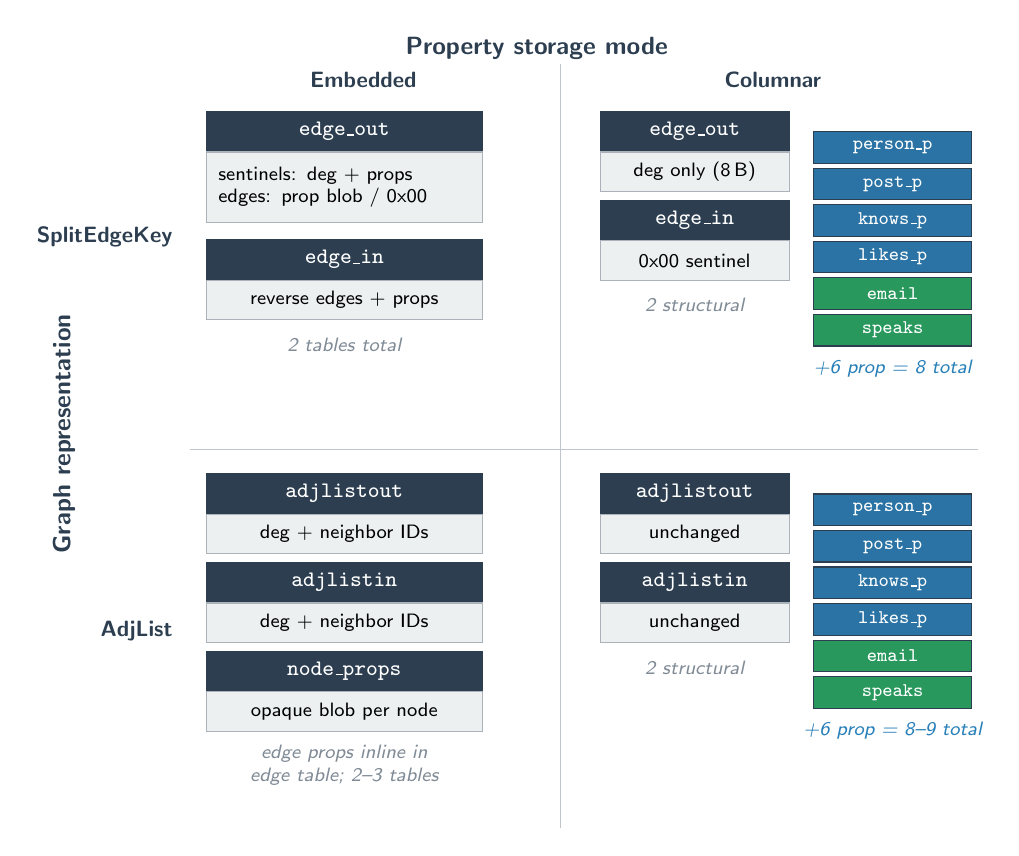
\begin{tikzpicture}

% ── Axis labels ─────────────────────────────────────────────────
\node[font=\sffamily\bfseries\small, text=tblheader, rotate=90]
  at (-1.8, -4.5) {Graph representation};
\node[font=\sffamily\bfseries\small, text=tblheader]
  at (4.2, 0.4) {Property storage mode};

% ── Column headers ──────────────────────────────────────────────
\node[font=\sffamily\bfseries\footnotesize, text=tblheader] at (2, 0) {Embedded};
\node[font=\sffamily\bfseries\footnotesize, text=tblheader] at (7.2, 0) {Columnar};

% ── Row headers ─────────────────────────────────────────────────
\node[font=\sffamily\bfseries\footnotesize, text=tblheader, anchor=east]
  at (-0.3, -2.0) {SplitEdgeKey};
\node[font=\sffamily\bfseries\footnotesize, text=tblheader, anchor=east]
  at (-0.3, -7.0) {AdjList};

% ════════════════════════════════════════════════════════════════════
%  QUADRANT 1: SplitEdgeKey Embedded  (top-left)
% ════════════════════════════════════════════════════════════════════
\node[tblhdr=35mm, anchor=north west] at (0, -0.4) (q1-eo)
  {\texttt{edge\_out}};
\node[tblcell=35mm, below=0mm of q1-eo, align=left, text width=32mm,
      minimum height=9mm] (q1-eo-body)
  {sentinels: deg + props\\edges: prop blob / 0x00};

\node[tblhdr=35mm, below=2mm of q1-eo-body] (q1-ei)
  {\texttt{edge\_in}};
\node[tblcell=35mm, below=0mm of q1-ei, minimum height=5mm] (q1-ei-body)
  {reverse edges + props};

\node[font=\sffamily\scriptsize\itshape, text=tblheader!60,
      below=1mm of q1-ei-body] {2 tables total};

% ════════════════════════════════════════════════════════════════════
%  QUADRANT 2: SplitEdgeKey Columnar  (top-right)
% ════════════════════════════════════════════════════════════════════
\node[tblhdr=24mm, anchor=north west] at (5, -0.4) (q2-eo)
  {\texttt{edge\_out}};
\node[tblcell=24mm, below=0mm of q2-eo, minimum height=5mm] (q2-eo-body)
  {deg only (8\,B)};

\node[tblhdr=24mm, below=1mm of q2-eo-body] (q2-ei)
  {\texttt{edge\_in}};
\node[tblcell=24mm, below=0mm of q2-ei, minimum height=5mm] (q2-ei-body)
  {0x00 sentinel};

\node[font=\sffamily\scriptsize\itshape, text=tblheader!60,
      below=1mm of q2-ei-body] (q2-struct-label) {2 structural};

% Property table pills — right of structural, within quadrant bounds
\coordinate (q2-prop-start) at ($(q2-eo.east) + (3mm, 0)$);
\node[tblhdr=20mm, minimum height=4mm, anchor=north west,
      fill=propClr!80!tblheader]
  at (q2-prop-start) (q2-pp)
  {\texttt{\scriptsize person\_p}};
\node[tblhdr=20mm, minimum height=4mm, below=0.5mm of q2-pp,
      fill=propClr!80!tblheader]
  (q2-po) {\texttt{\scriptsize post\_p}};
\node[tblhdr=20mm, minimum height=4mm, below=0.5mm of q2-po,
      fill=propClr!80!tblheader]
  (q2-kp) {\texttt{\scriptsize knows\_p}};
\node[tblhdr=20mm, minimum height=4mm, below=0.5mm of q2-kp,
      fill=propClr!80!tblheader]
  (q2-lp) {\texttt{\scriptsize likes\_p}};
\node[tblhdr=20mm, minimum height=4mm, below=0.5mm of q2-lp,
      fill=secClr!80!tblheader]
  (q2-pe) {\texttt{\scriptsize email}};
\node[tblhdr=20mm, minimum height=4mm, below=0.5mm of q2-pe,
      fill=secClr!80!tblheader]
  (q2-ps) {\texttt{\scriptsize speaks}};

\node[font=\sffamily\scriptsize\itshape, text=propClr,
      below=0.5mm of q2-ps] (q2-prop-label) {+6 prop = 8 total};

% ════════════════════════════════════════════════════════════════════
%  QUADRANT 3: AdjList Embedded  (bottom-left)
% ════════════════════════════════════════════════════════════════════
\node[tblhdr=35mm, anchor=north west] at (0, -5.0) (q3-ao)
  {\texttt{adjlistout}};
\node[tblcell=35mm, below=0mm of q3-ao, minimum height=5mm] (q3-ao-body)
  {deg + neighbor IDs};

\node[tblhdr=35mm, below=1mm of q3-ao-body] (q3-ai)
  {\texttt{adjlistin}};
\node[tblcell=35mm, below=0mm of q3-ai, minimum height=5mm] (q3-ai-body)
  {deg + neighbor IDs};

\node[tblhdr=35mm, below=1mm of q3-ai-body] (q3-np)
  {\texttt{node\_props}};
\node[tblcell=35mm, below=0mm of q3-np, minimum height=5mm] (q3-np-body)
  {opaque blob per node};

\node[font=\sffamily\scriptsize, below=0.5mm of q3-np-body, text width=34mm,
      align=center, text=tblheader!60]
  (q3-label) {\itshape edge props inline in\\edge table; 2--3 tables};

% ════════════════════════════════════════════════════════════════════
%  QUADRANT 4: AdjList Columnar  (bottom-right)
% ════════════════════════════════════════════════════════════════════
\node[tblhdr=24mm, anchor=north west] at (5, -5.0) (q4-ao)
  {\texttt{adjlistout}};
\node[tblcell=24mm, below=0mm of q4-ao, minimum height=5mm] (q4-ao-body)
  {unchanged};

\node[tblhdr=24mm, below=1mm of q4-ao-body] (q4-ai)
  {\texttt{adjlistin}};
\node[tblcell=24mm, below=0mm of q4-ai, minimum height=5mm] (q4-ai-body)
  {unchanged};

\node[font=\sffamily\scriptsize\itshape, text=tblheader!60,
      below=1mm of q4-ai-body] (q4-struct-label) {2 structural};

% Property table pills — right of structural, within quadrant bounds
\coordinate (q4-prop-start) at ($(q4-ao.east) + (3mm, 0)$);
\node[tblhdr=20mm, minimum height=4mm, anchor=north west,
      fill=propClr!80!tblheader]
  at (q4-prop-start) (q4-pp)
  {\texttt{\scriptsize person\_p}};
\node[tblhdr=20mm, minimum height=4mm, below=0.5mm of q4-pp,
      fill=propClr!80!tblheader]
  (q4-po) {\texttt{\scriptsize post\_p}};
\node[tblhdr=20mm, minimum height=4mm, below=0.5mm of q4-po,
      fill=propClr!80!tblheader]
  (q4-kp) {\texttt{\scriptsize knows\_p}};
\node[tblhdr=20mm, minimum height=4mm, below=0.5mm of q4-kp,
      fill=propClr!80!tblheader]
  (q4-lp) {\texttt{\scriptsize likes\_p}};
\node[tblhdr=20mm, minimum height=4mm, below=0.5mm of q4-lp,
      fill=secClr!80!tblheader]
  (q4-pe) {\texttt{\scriptsize email}};
\node[tblhdr=20mm, minimum height=4mm, below=0.5mm of q4-pe,
      fill=secClr!80!tblheader]
  (q4-ps) {\texttt{\scriptsize speaks}};

\node[font=\sffamily\scriptsize\itshape, text=propClr,
      below=0.5mm of q4-ps] {+6 prop = 8--9 total};

% ── Dividing lines ──────────────────────────────────────────────
\draw[tblheader!30, line width=0.4pt]
  (4.5, 0.2) -- (4.5, -9.5);
\draw[tblheader!30, line width=0.4pt]
  (-0.2, -4.7) -- (9.8, -4.7);

\end{tikzpicture}
\end{document}
